\section{Letter Font Application}
\label{sec:font}
This section presents letter font model GUI application, the inputs comes from a user, and user can choose a set of settings, the main one is the font, font style, size of letter. This application writes a set of drilling points in to txt file, the txt file also can choose arbitrary a user. The letter font model is implemented under vision (image processing), so all theory from image processing could be applied there.\\
The purpose of this application is to return letters drilling points, and these drilling points would be used to performing drilling (carving) by robot arm Fanuc 200ib (figure \ref{fig:writingbox}).

\begin{figure}[H]
  \centering
  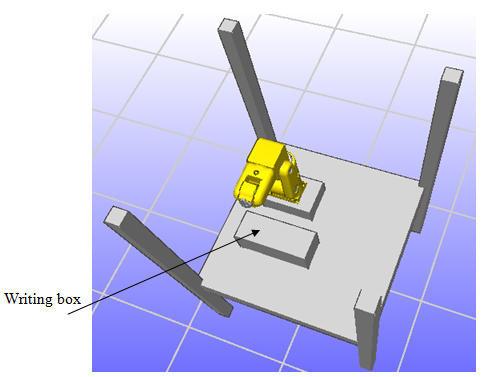
\includegraphics[scale= 1]{source/writingbox.png}
  \caption{Writing box position}
  \label{fig:writingbox}
\end{figure}

Letter font model is an important step for performing actual (real) letter carving on foam, another step would be inverse kinematics, which path planner uses for planning movements between frames. The application main window is shown in figure  \ref{fig:letterapp}, also there is provided a description of application elements.

\begin{figure}[H]
  \centering
  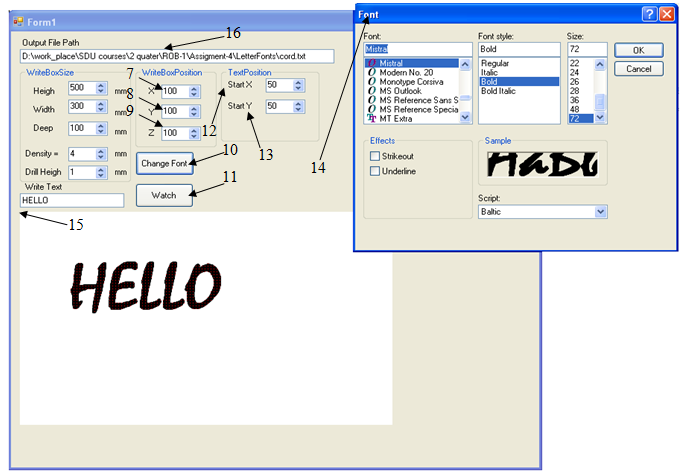
\includegraphics[scale= 0.8]{source/letterapp.png}
  \caption{Letter font application}
  \label{fig:letterapp}
\end{figure}

\begin{enumerate}
\item Sets writing box height
\item Sets writing box width
\item Sets writing box deep
\item Set the density of drilling points (red points)
\item Sets the drill height, in other words, how deep we want to drill
\item The place of letter or text
\item Set the writing box position according X coordinate (in Cartesian domain)
\item Set the writing box position according Y coordinate (in Cartesian domain)
\item Set the writing box position according Z coordinate (in Cartesian domain) 
\item Call the font window
\item Display the text on writing box
\item Set the text position according X (in Cartesian domain) on writing box
\item Set the text position according Y (in Cartesian domain) on writing box
\item The font window, where we can the size, font, font style of text
\item The start position of writing box
\item The path of txt file, where are stored each drilling points
\end{enumerate}

First by application we set the txt file path, the txt file stores each drilling points information, this information we can see also in C\# application (figure \ref{fig:letterconsole}). Second it is necessary to set writing box position, because according this position would be wrote drilling points, and other settings are optional. 

\begin{figure}[H]
  \centering
  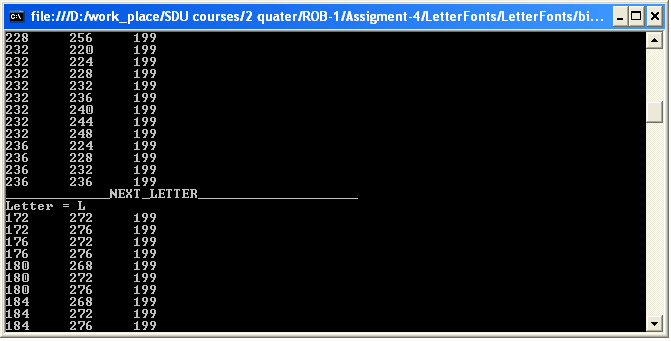
\includegraphics[scale= 0.6]{source/letterconsole.png}
  \caption{Letter font application console}
  \label{fig:letterconsole}
\end{figure}

As we can see from figure \ref{fig:letterconsole} each letter’s drilling point are separated, because the image is consider as a set of letters. We could do not separate the letters, but then it would be consider as a set of drilling positions, and we would not be able carving out letters, just drilling. We could react or take some actions then the letter’s drilling points finish, or skip it.

\subsection{Letter labeling application}
We deal with image in byte mode and the image is represented like figure \ref{fig:imagebyte}. As we can see the image is composed of R-red, G-green, B-blue bytes and padding bytes. We are interesting only in RGB bytes, the padding bytes describe how image is stored in memory, and they do not have any influence of displaying image. The programming becomes complex, because in order to jump to next image’s row we need count offset (which is equal (stride – images width)), and in order to access to next pixel we need to jump by three bytes.

\begin{figure}[H]
  \centering
  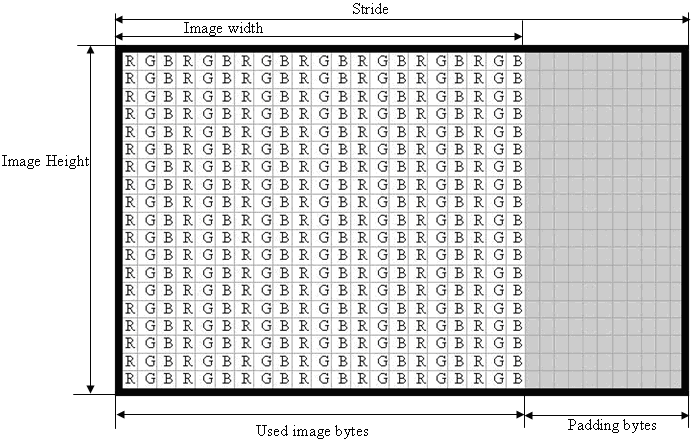
\includegraphics[scale= 0.6]{source/imagebyte.png}
  \caption{Image in byte mode}
  \label{fig:imagebyte}
\end{figure}

We deal with two images, one image is an original, and another image is was a clone of original image. In clone image we access to each pixel bytes, and use such image as an array, where we change values, we do it in such way because it is faster, and easier access to write values, rather than to create a huge array, and write by own functions.

 Was used 9 pixels connectivity matrix figure  \ref{fig:pixelmatrix}, there are a lot of options but we chose such one, it is not too big, by the way and easy manages such shape of matrix (not like triangles or cross shape).  

\begin{figure}[H]
  \centering
  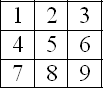
\includegraphics[scale= 0.6]{source/pixelmatrix.png}
  \caption{9 pixels’ connectivity matrix}
  \label{fig:pixelmatrix}
\end{figure}

Connectivity matrix is used to take values from original image and write the result to a clone image. Another reason of choosing 3x3 connectivity matrix is what we loose only images corners pixels. It was possibility to choose 2x2 matrix, but the time of image processing would significantly increase, and we would also loose also the corner pixels.

\begin{figure}[H]
  \centering
  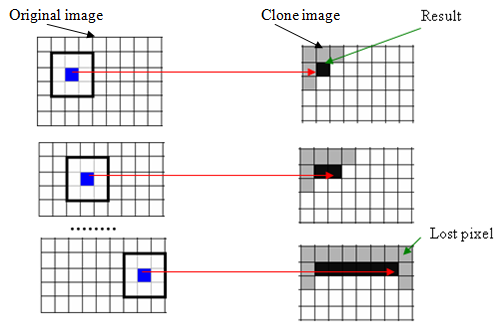
\includegraphics[scale= 0.6]{source/matriximages.png}
  \caption{9 pixels’ connectivity matrix over image}
  \label{fig:matriximages}
\end{figure}

The letters (objects) labeling algorithm is shown in figure \ref{fig:matriximages}. At the beginning the image is converted to binary, it allow us easier to deal with information, we set non-white pixels to black. 

\begin{figure}[H]
  \centering
  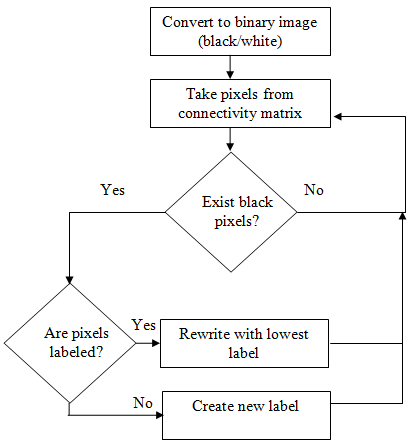
\includegraphics[scale= 0.6]{source/labeling.png}
  \caption{Letters labeling algorithm}
  \label{fig:labeling}
\end{figure}

When we have a binary image we have only two values: black – which represent the letter (or object), and white – which we assume as background. In the next step we take pixels from connectivity matrix and check if exists black pixels (which belongs to letter or object), if there are no black pixels we move the connectivity matrix by one pixel in particular direction and repeat the black pixel checking. But if there are black pixels, we perform checking in order to figure out or we need to create a new label (detected new object) or some of these pixels belongs to before detected letter (or object), and it is enough to rewrite the previous labels. The example of labeling text letters is shown in figure \ref{fig:labelingexample}. We have a binary image this image is called “clone image” it is a copy of original.  By performing letters labeling algorithm (figure \ref{fig:labeling}) we can detect how much different letters (objects) we have. The important thing is what we should twice repeat letters labeling algorithm, at first time we arbitrary choose from which images corner to start, for instance it  is convenient to start  from the top/left corner, the second time of repeating algorithm we need to choose an opposite corner it would be bottom/right.

\begin{figure}[H]
  \centering
  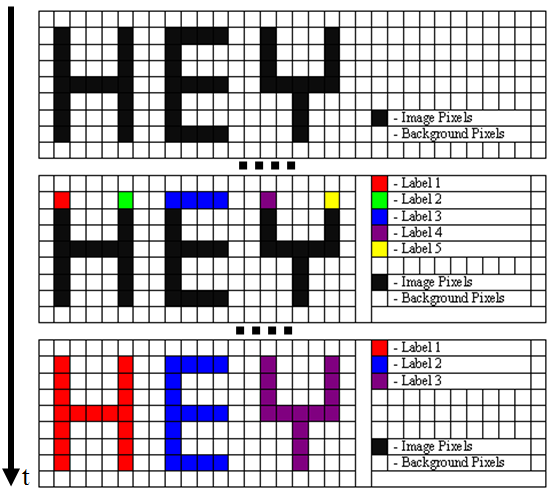
\includegraphics[scale= 0.6]{source/labelingexample.png}
  \caption{Letters labeling example}
  \label{fig:labelingexample}
\end{figure}

If we would not perform algorithm from opposite corner, the algorithm would detect more letters (objects) then there exists, in such letters as U, Y, H, V, W … , because the connectivity matrix is too small, but if we choose connectivity matrix quite large, there are risks: detect two letters as one letter, loose more pixels (near image corners).

\subsection{Letter Font Application Extension}
At the moment the letter font application deals with text as an image, in other words, the letters are consider as image (which we can save, paint, change color).  So it is possible to load image directly (this feature is not implemented on final application, because the task was to deal with letters), so by having this application source code and knowing basics of objecting oriented programming, it easy to load any picture here as shown in figure \ref{fig:letterappextension}.   

\begin{figure}[H]
  \centering
  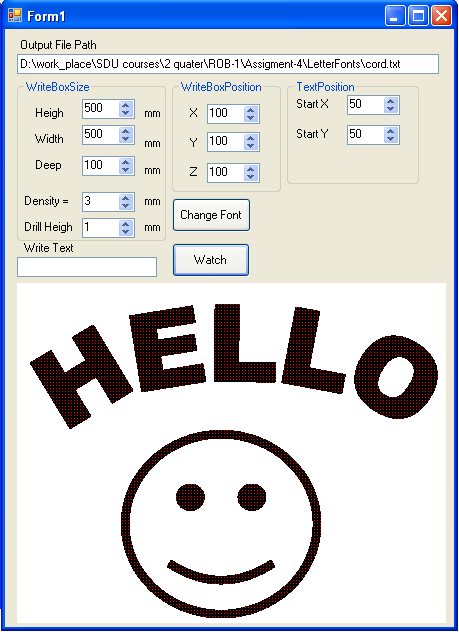
\includegraphics[scale= 0.6]{source/letterappextension.png}
  \caption{Letter font application}
  \label{fig:letterappextension}
\end{figure}

The interesting thing is what all image processing knowledge we could apply here, such as edge detection, Hough transformation etc., and this is mean what this letter font application is universal, we can easy make extensions.  
